%=====================================================================
\section{The wall lattice in circles}\label{sec:clattice}
Fourier analysis of the wall-sign defects along the wall (methods: Secs.~\ref{sec:md-fourier-static}, \ref{sec:md-fourier-dyn}):
lattice period $m^*$, occupancy $N_\mathrm{wall}/m_\mathrm{lat}$, instantaneous order $S(m^*)/N_\mathrm{wall}$ (1 = perfect
lattice in every frame, even if it moves), static fraction $f_\mathrm{static}$ (1 = the lattice sits at fixed sites), lattice
memory $F(m^*,1000)$ in the co-moving frame (1 = pinned or rigidly sliding), rearrangement time $\tau_\mathrm{fl}$ and the
sliding speed. 930 circle runs, $\rho\le0.15$, both signs, 3 seeds.
\begin{figure}[H]\centering
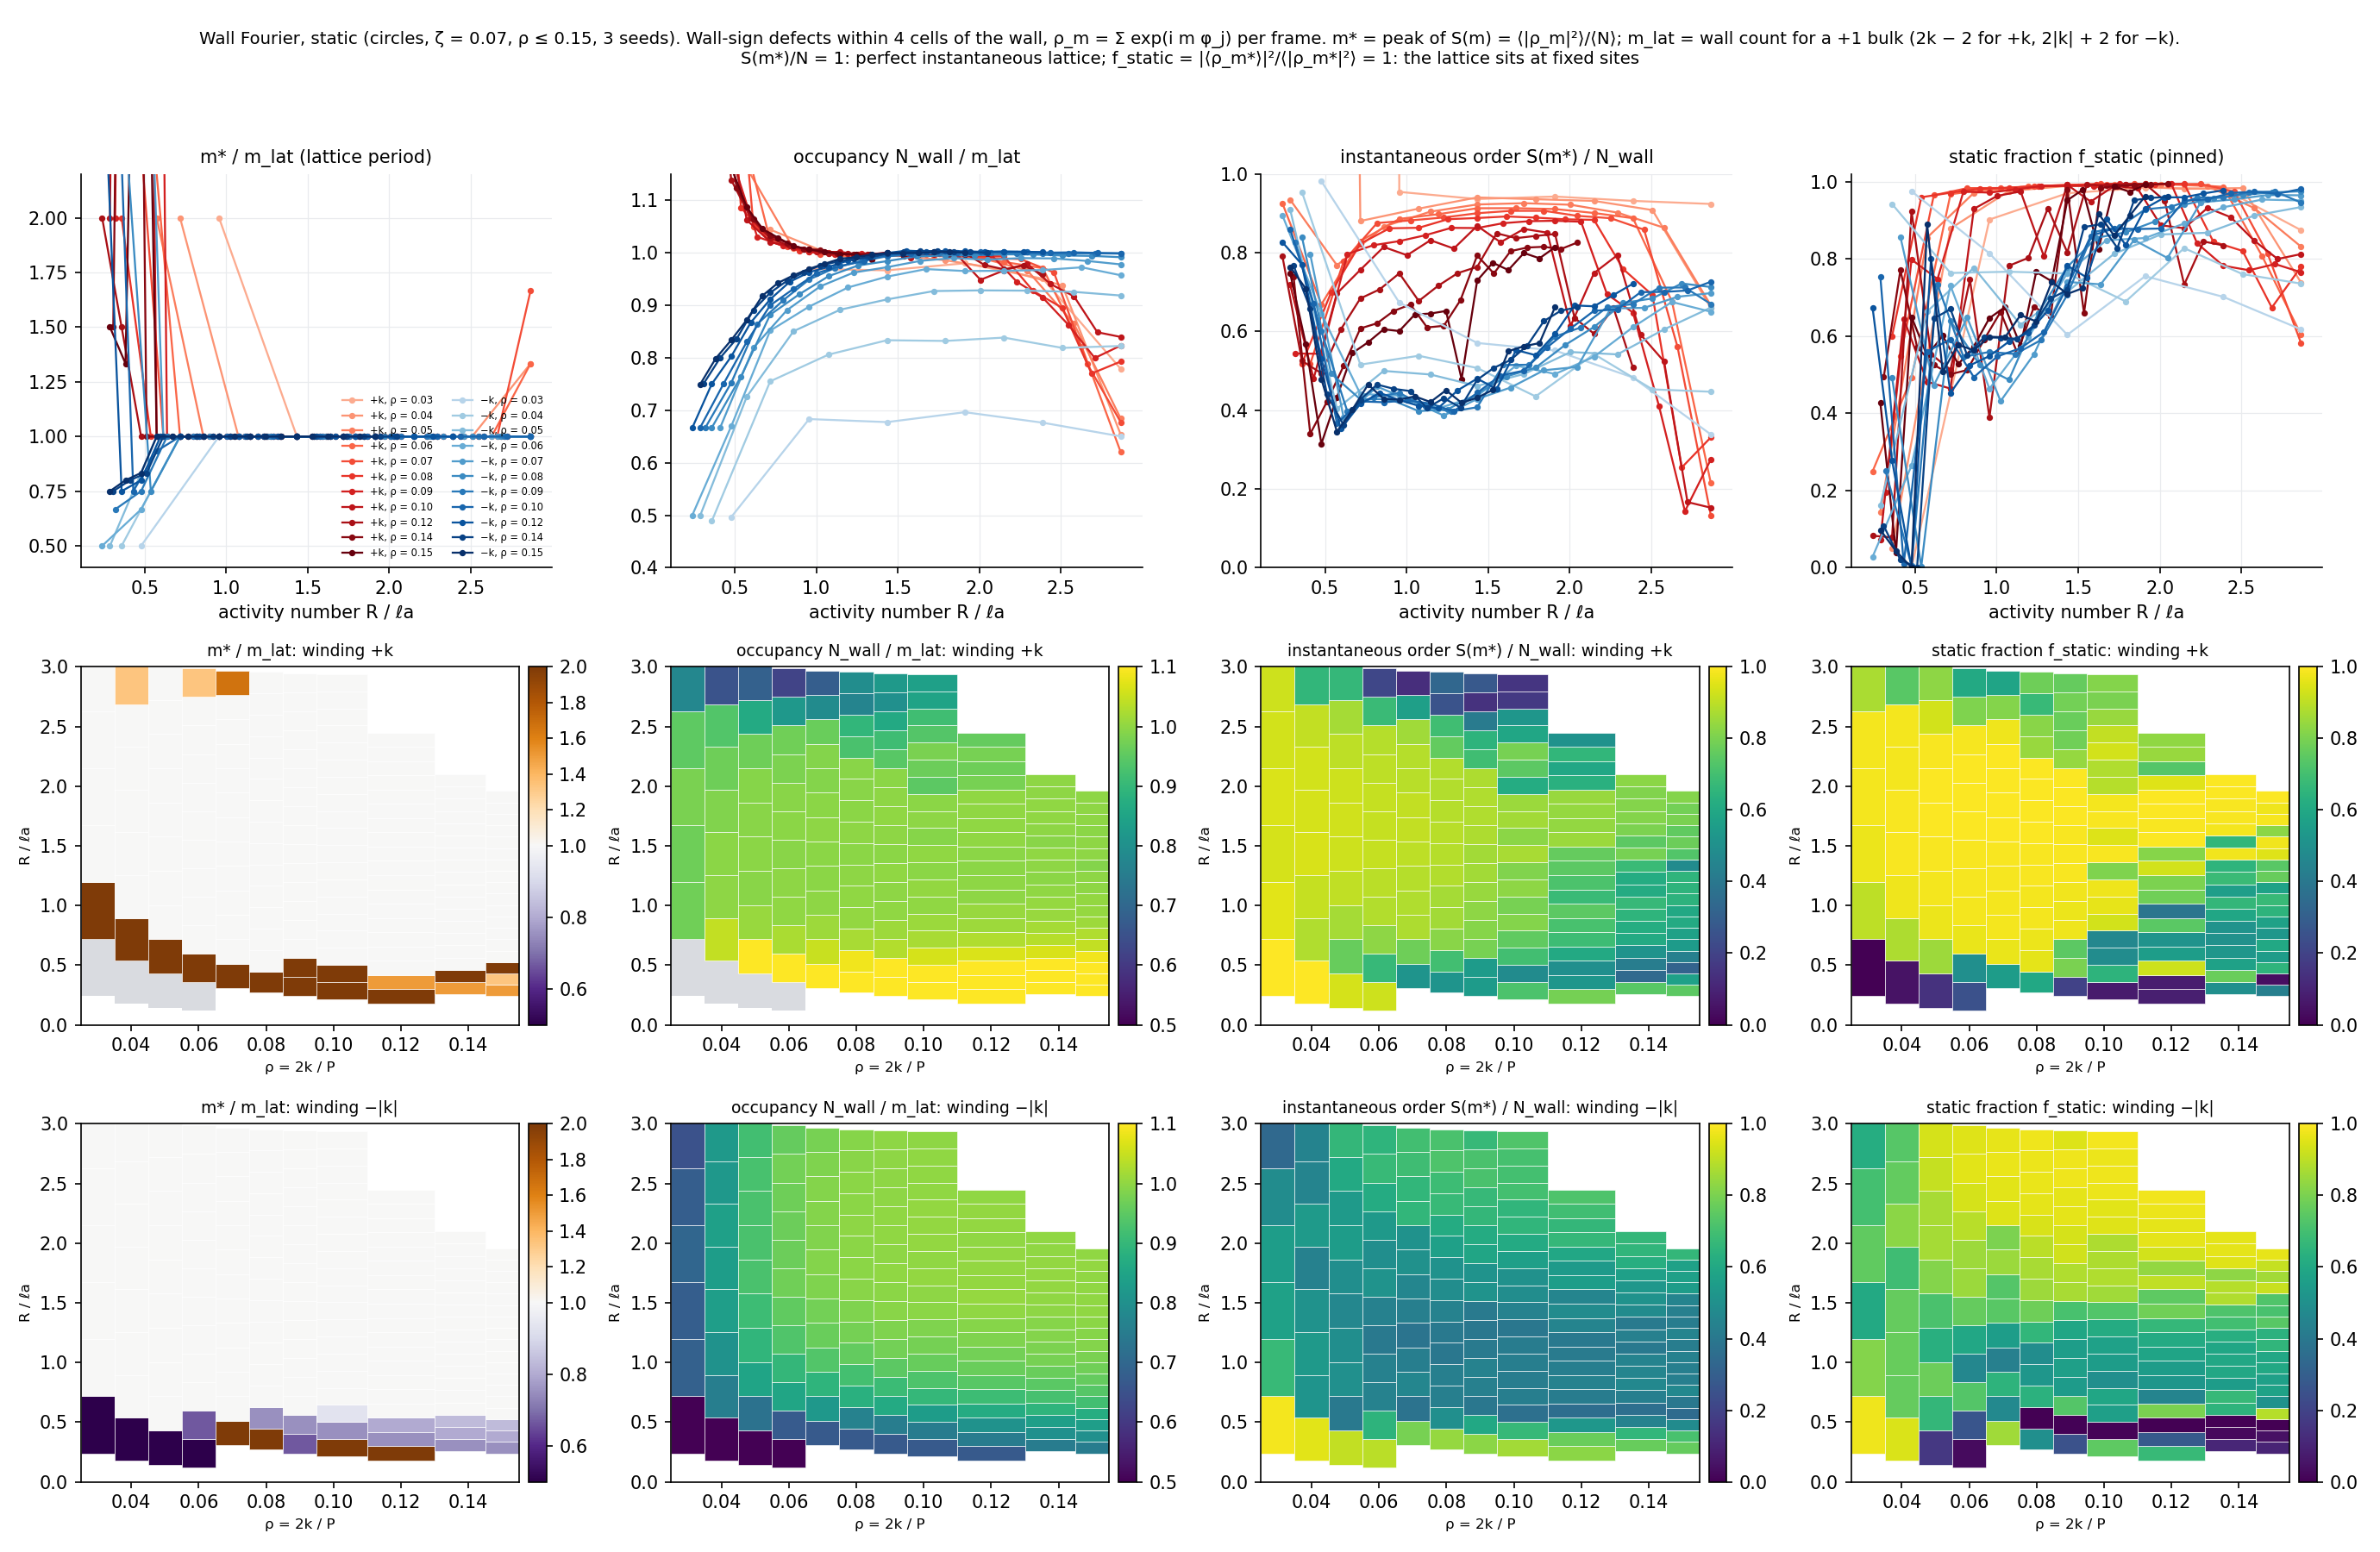
\includegraphics[width=\textwidth]{fourier_static_circles.png}
\caption{Static wall Fourier analysis of the circles. Columns: $m^*/m_\mathrm{lat}$ (with $m_\mathrm{lat}=2k-2$ for $+k$,
$2|k|+2$ for $-k$, the wall count of a $+1$ bulk), occupancy, instantaneous order, static fraction. Top: against $R/\la$,
one curve per $\rho$ (red $+k$, blue $-|k|$); middle and bottom: maps for $+k$ and $-|k|$.}\label{fig:fstat}
\end{figure}
\begin{figure}[H]\centering
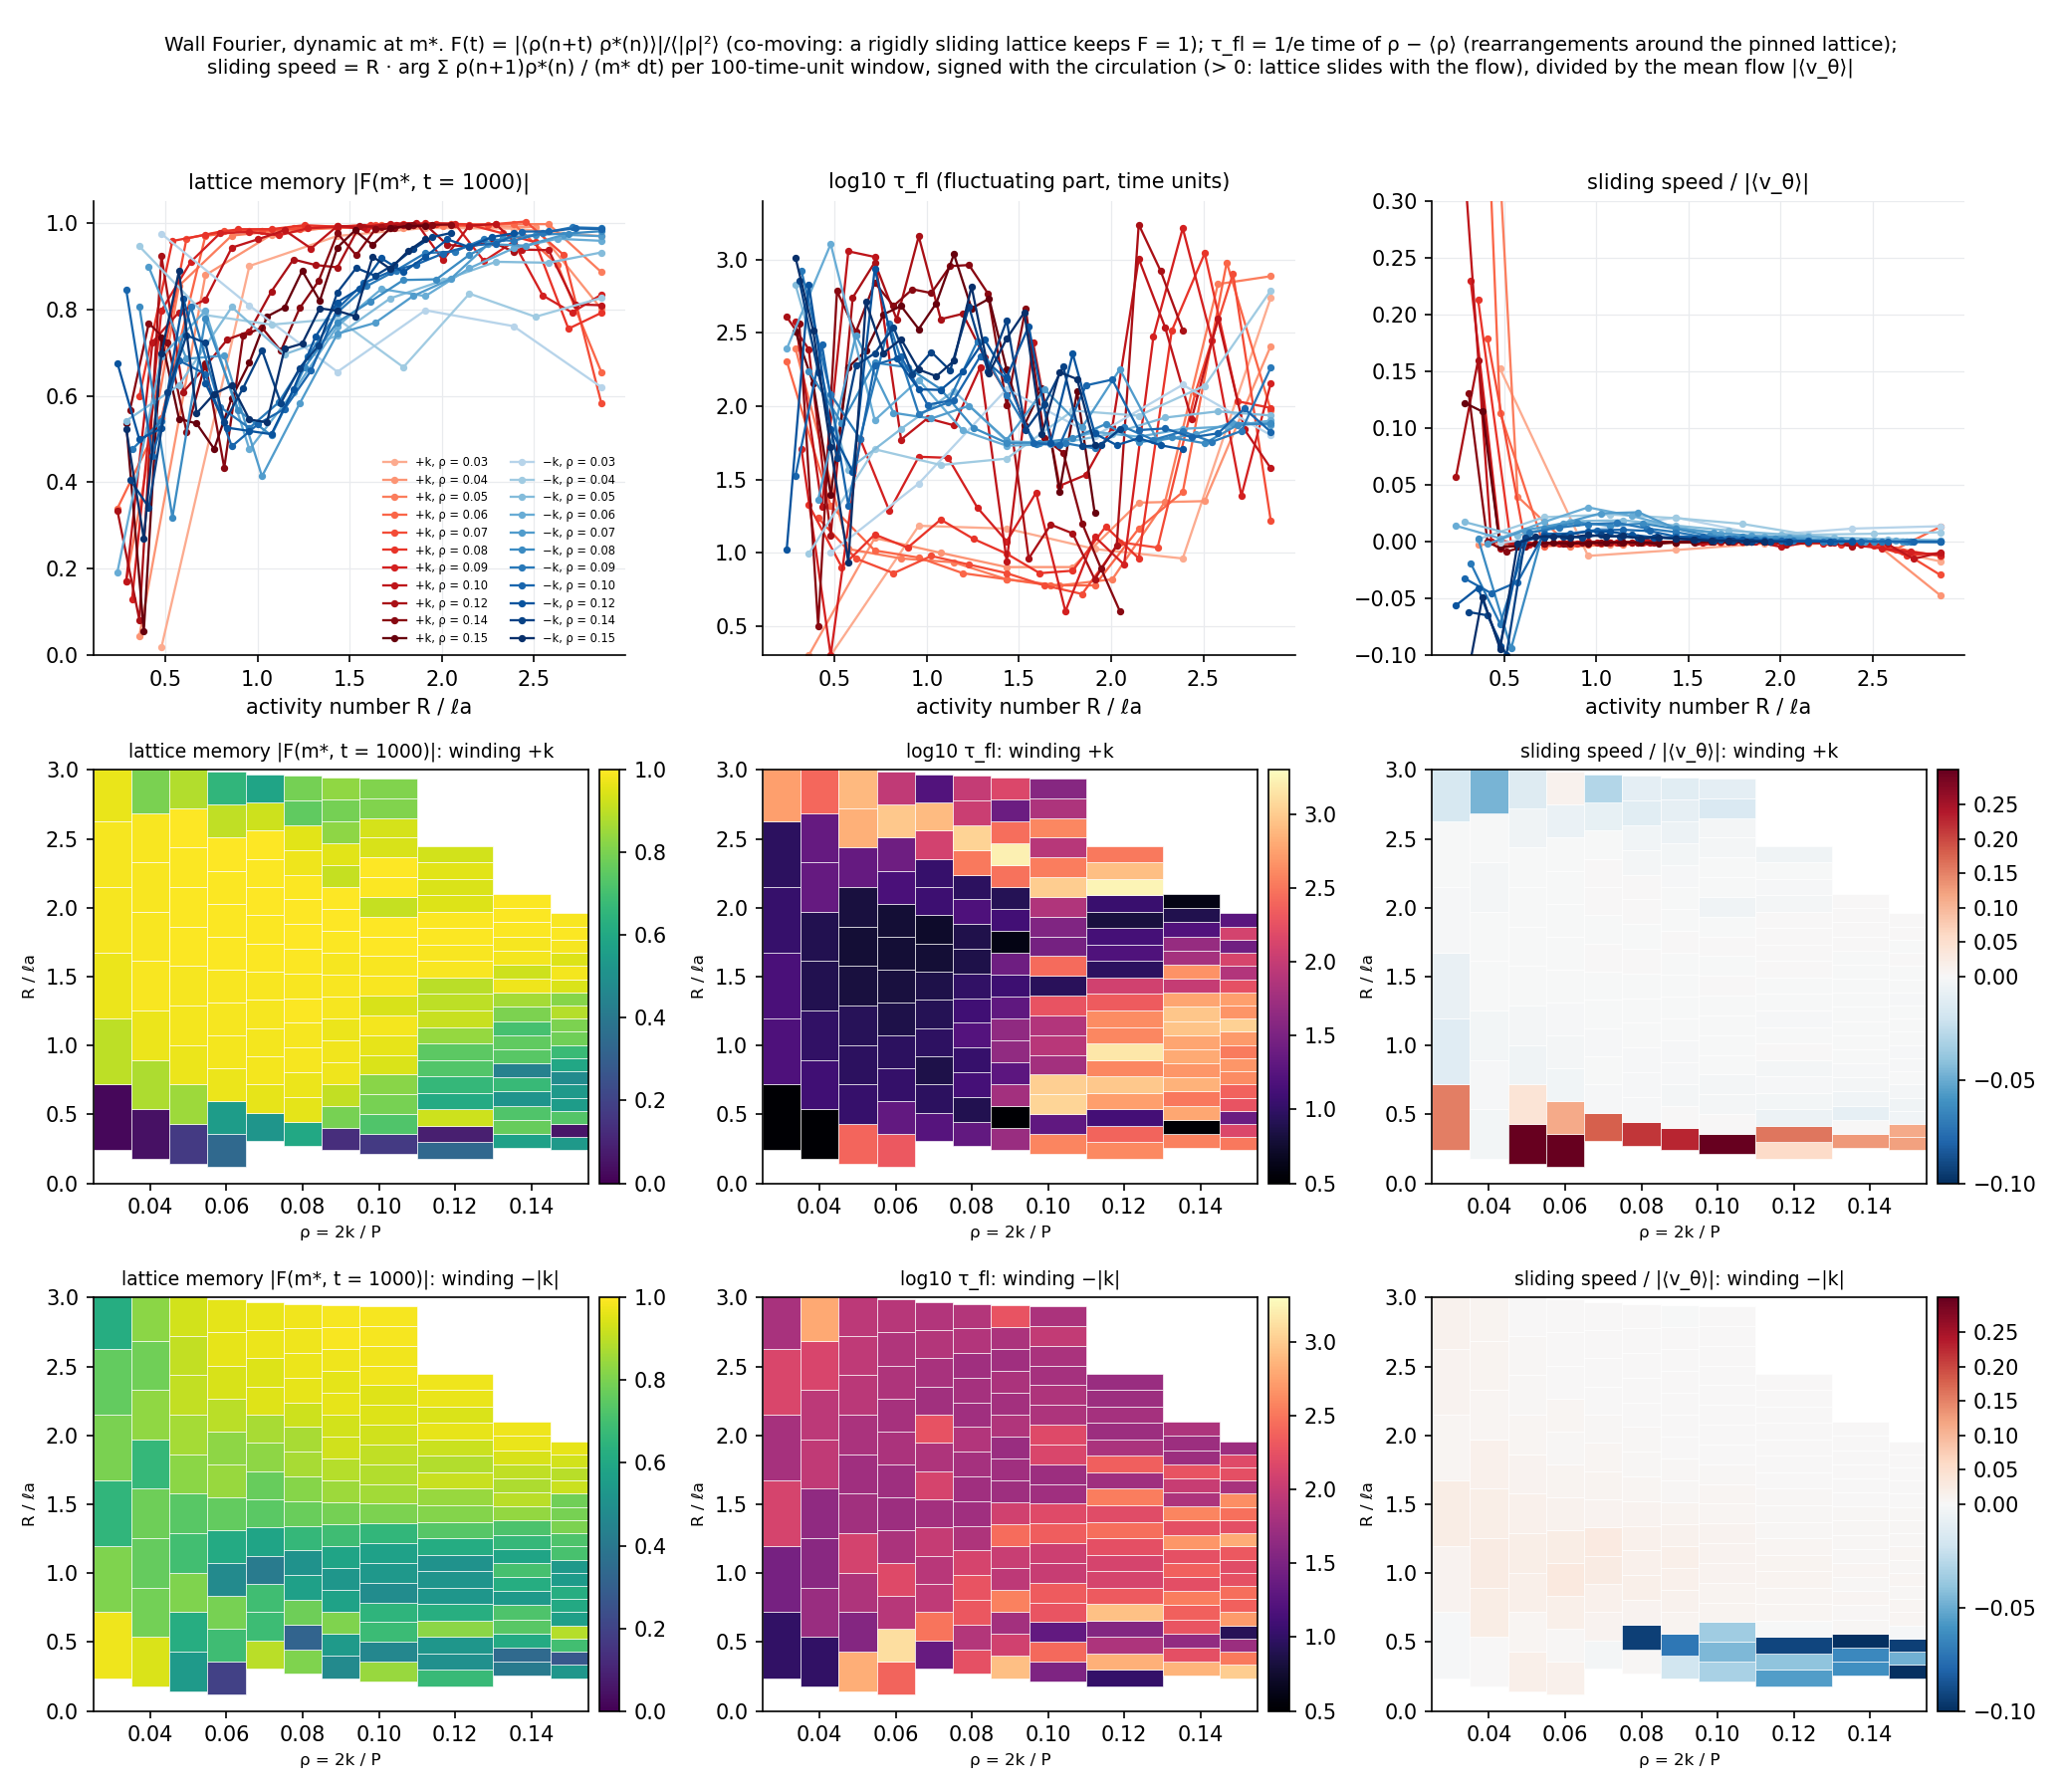
\includegraphics[width=0.9\textwidth]{fourier_dynamic_circles.png}
\caption{Dynamic wall Fourier analysis: lattice memory $|F(m^*,t=1000)|$, $\log_{10}\tau_\mathrm{fl}$ (rearrangements around the
pinned lattice) and the sliding speed divided by the mean flow $|\langle v_\theta\rangle|$ (positive: with the flow).}\label{fig:fdyn}
\end{figure}
\begin{itemize}
  \item \textbf{Period.} $m^*=m_\mathrm{lat}$ in every run with $R\gtrsim0.5$--$0.75\,\la$, for both signs: the wall lattice
        always has the period of a $+1$ bulk, $2k-2$ sites for $+k$ and $2|k|+2$ for $-k$.
  \item \textbf{Occupancy.} $+k$: 1.0 from 0.75 to $2.3\,\la$, dropping to 0.6--0.85 at $R\gtrsim2.5\,\la$ (layer loss).
        $-k$: 0.7--0.9 at low $\rho$, rising to 1 at high $\rho$ or large $|k|$ --- the vacancies that keep the mirror bulk below $+1$.
  \item \textbf{Order and pinning.} $+k$: $S/N=0.8$--0.9 at low $\rho$, 0.5--0.8 at high $\rho$; $f_\mathrm{static}\approx0.95$--1.
        $-k$: $S/N$ only 0.4--0.6, $f_\mathrm{static}$ 0.5--0.9, rising with $R$.
  \item \textbf{No sliding.} Lattice speed $<2$--3\% of $|\langle v_\theta\rangle|$ for $R>0.6\,\la$; only tiny cavities rotate.
        Lattice memory $\approx1$ for $+k$ in the layer window, 0.5--0.9 for $-k$. Rearrangement time $\tau_\mathrm{fl}\sim10$
        time units for $+k$ at low $\rho$, 100--1000 at high $\rho$, 60--100 for $-k$. \textbf{The layer is pinned, or vacant and
        melting; an ordered layer sliding with the vortex never occurs.} The earlier impression of a ``partly sliding'' layer at
        $2.87\,\la$ (static fraction 0.87) is vacancies, not sliding.
  \item \textbf{Per-defect drift} (Sec.~\ref{sec:md-drift}; $k=6$ circles analysed with the oval script): drift/$|v_w|\approx0$
        ($<1\%$) for $R=0.7$--$1.7\,\la$, $-2\%$ at $2.15\,\la$, $-18\%$ at $2.87\,\la$ (occupancy 0.78): in circles the wall defects
        move against the flow only where the lattice has vacancies (compare ovals, Sec.~\ref{sec:slattice}).
\end{itemize}
